\PassOptionsToPackage{unicode=true}{hyperref} % options for packages loaded elsewhere
\PassOptionsToPackage{hyphens}{url}
%
\documentclass[]{article}
\usepackage{lmodern}
\usepackage{amssymb,amsmath}
\usepackage{ifxetex,ifluatex}
\usepackage{fixltx2e} % provides \textsubscript
\ifnum 0\ifxetex 1\fi\ifluatex 1\fi=0 % if pdftex
  \usepackage[T1]{fontenc}
  \usepackage[utf8]{inputenc}
  \usepackage{textcomp} % provides euro and other symbols
\else % if luatex or xelatex
  \usepackage{unicode-math}
  \defaultfontfeatures{Ligatures=TeX,Scale=MatchLowercase}
\fi
% use upquote if available, for straight quotes in verbatim environments
\IfFileExists{upquote.sty}{\usepackage{upquote}}{}
% use microtype if available
\IfFileExists{microtype.sty}{%
\usepackage[]{microtype}
\UseMicrotypeSet[protrusion]{basicmath} % disable protrusion for tt fonts
}{}
\IfFileExists{parskip.sty}{%
\usepackage{parskip}
}{% else
\setlength{\parindent}{0pt}
\setlength{\parskip}{6pt plus 2pt minus 1pt}
}
\usepackage{hyperref}
\hypersetup{
            pdftitle={Class8},
            pdfauthor={Rimma Levina},
            pdfborder={0 0 0},
            breaklinks=true}
\urlstyle{same}  % don't use monospace font for urls
\usepackage[margin=1in]{geometry}
\usepackage{color}
\usepackage{fancyvrb}
\newcommand{\VerbBar}{|}
\newcommand{\VERB}{\Verb[commandchars=\\\{\}]}
\DefineVerbatimEnvironment{Highlighting}{Verbatim}{commandchars=\\\{\}}
% Add ',fontsize=\small' for more characters per line
\usepackage{framed}
\definecolor{shadecolor}{RGB}{248,248,248}
\newenvironment{Shaded}{\begin{snugshade}}{\end{snugshade}}
\newcommand{\AlertTok}[1]{\textcolor[rgb]{0.94,0.16,0.16}{#1}}
\newcommand{\AnnotationTok}[1]{\textcolor[rgb]{0.56,0.35,0.01}{\textbf{\textit{#1}}}}
\newcommand{\AttributeTok}[1]{\textcolor[rgb]{0.77,0.63,0.00}{#1}}
\newcommand{\BaseNTok}[1]{\textcolor[rgb]{0.00,0.00,0.81}{#1}}
\newcommand{\BuiltInTok}[1]{#1}
\newcommand{\CharTok}[1]{\textcolor[rgb]{0.31,0.60,0.02}{#1}}
\newcommand{\CommentTok}[1]{\textcolor[rgb]{0.56,0.35,0.01}{\textit{#1}}}
\newcommand{\CommentVarTok}[1]{\textcolor[rgb]{0.56,0.35,0.01}{\textbf{\textit{#1}}}}
\newcommand{\ConstantTok}[1]{\textcolor[rgb]{0.00,0.00,0.00}{#1}}
\newcommand{\ControlFlowTok}[1]{\textcolor[rgb]{0.13,0.29,0.53}{\textbf{#1}}}
\newcommand{\DataTypeTok}[1]{\textcolor[rgb]{0.13,0.29,0.53}{#1}}
\newcommand{\DecValTok}[1]{\textcolor[rgb]{0.00,0.00,0.81}{#1}}
\newcommand{\DocumentationTok}[1]{\textcolor[rgb]{0.56,0.35,0.01}{\textbf{\textit{#1}}}}
\newcommand{\ErrorTok}[1]{\textcolor[rgb]{0.64,0.00,0.00}{\textbf{#1}}}
\newcommand{\ExtensionTok}[1]{#1}
\newcommand{\FloatTok}[1]{\textcolor[rgb]{0.00,0.00,0.81}{#1}}
\newcommand{\FunctionTok}[1]{\textcolor[rgb]{0.00,0.00,0.00}{#1}}
\newcommand{\ImportTok}[1]{#1}
\newcommand{\InformationTok}[1]{\textcolor[rgb]{0.56,0.35,0.01}{\textbf{\textit{#1}}}}
\newcommand{\KeywordTok}[1]{\textcolor[rgb]{0.13,0.29,0.53}{\textbf{#1}}}
\newcommand{\NormalTok}[1]{#1}
\newcommand{\OperatorTok}[1]{\textcolor[rgb]{0.81,0.36,0.00}{\textbf{#1}}}
\newcommand{\OtherTok}[1]{\textcolor[rgb]{0.56,0.35,0.01}{#1}}
\newcommand{\PreprocessorTok}[1]{\textcolor[rgb]{0.56,0.35,0.01}{\textit{#1}}}
\newcommand{\RegionMarkerTok}[1]{#1}
\newcommand{\SpecialCharTok}[1]{\textcolor[rgb]{0.00,0.00,0.00}{#1}}
\newcommand{\SpecialStringTok}[1]{\textcolor[rgb]{0.31,0.60,0.02}{#1}}
\newcommand{\StringTok}[1]{\textcolor[rgb]{0.31,0.60,0.02}{#1}}
\newcommand{\VariableTok}[1]{\textcolor[rgb]{0.00,0.00,0.00}{#1}}
\newcommand{\VerbatimStringTok}[1]{\textcolor[rgb]{0.31,0.60,0.02}{#1}}
\newcommand{\WarningTok}[1]{\textcolor[rgb]{0.56,0.35,0.01}{\textbf{\textit{#1}}}}
\usepackage{graphicx,grffile}
\makeatletter
\def\maxwidth{\ifdim\Gin@nat@width>\linewidth\linewidth\else\Gin@nat@width\fi}
\def\maxheight{\ifdim\Gin@nat@height>\textheight\textheight\else\Gin@nat@height\fi}
\makeatother
% Scale images if necessary, so that they will not overflow the page
% margins by default, and it is still possible to overwrite the defaults
% using explicit options in \includegraphics[width, height, ...]{}
\setkeys{Gin}{width=\maxwidth,height=\maxheight,keepaspectratio}
\setlength{\emergencystretch}{3em}  % prevent overfull lines
\providecommand{\tightlist}{%
  \setlength{\itemsep}{0pt}\setlength{\parskip}{0pt}}
\setcounter{secnumdepth}{0}
% Redefines (sub)paragraphs to behave more like sections
\ifx\paragraph\undefined\else
\let\oldparagraph\paragraph
\renewcommand{\paragraph}[1]{\oldparagraph{#1}\mbox{}}
\fi
\ifx\subparagraph\undefined\else
\let\oldsubparagraph\subparagraph
\renewcommand{\subparagraph}[1]{\oldsubparagraph{#1}\mbox{}}
\fi

% set default figure placement to htbp
\makeatletter
\def\fps@figure{htbp}
\makeatother


\title{Class8}
\author{Rimma Levina}
\date{2/5/2020}

\begin{document}
\maketitle

\hypertarget{k-means-clustering}{%
\subsection{K-means clustering}\label{k-means-clustering}}

Lets try the \texttt{kmeans()} function in R to cluster some made up
example data

\begin{Shaded}
\begin{Highlighting}[]
\NormalTok{tmp <-}\StringTok{ }\KeywordTok{c}\NormalTok{(}\KeywordTok{rnorm}\NormalTok{(}\DecValTok{30}\NormalTok{,}\OperatorTok{-}\DecValTok{3}\NormalTok{), }\KeywordTok{rnorm}\NormalTok{(}\DecValTok{30}\NormalTok{,}\DecValTok{3}\NormalTok{)) }\CommentTok{#this makes up data, 1st = 30 points centered around -3, 2nd = 30 points centered around +3 --> makes a vector that has 60 points}

\NormalTok{x <-}\StringTok{ }\KeywordTok{cbind}\NormalTok{(}\DataTypeTok{x=}\NormalTok{tmp, }\DataTypeTok{y=}\KeywordTok{rev}\NormalTok{(tmp)) }\CommentTok{# cbind() binds together vectors, you are also setting the axes, where x is the first vector and y is the reverse (rev()) of the tmp vector, then you plot and see you have 2 groups that are clearly separate/clustered}
 
\KeywordTok{plot}\NormalTok{(x)}
\end{Highlighting}
\end{Shaded}

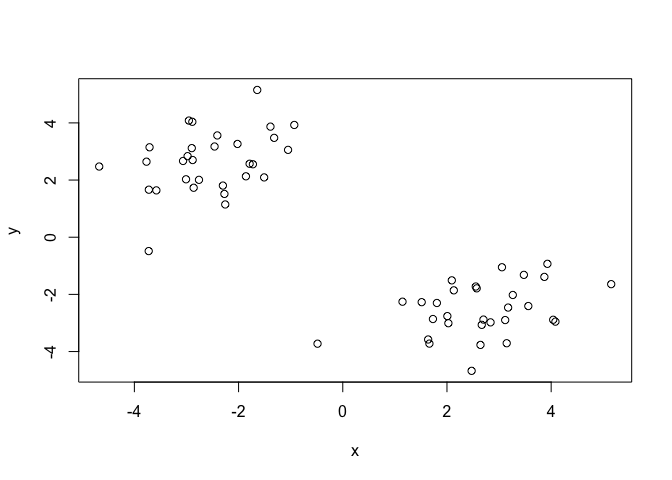
\includegraphics{Class-8_files/figure-latex/unnamed-chunk-1-1.pdf} Use
the kmeans() function setting k to 2 and nstart=20 Inspect/print the
results Q. How many points are in each cluster? Q. What `component' of
your result object details - cluster size?\\
- cluster assignment/membership?\\
- cluster center?

Plot x colored by the kmeans cluster assignment and add cluster centers
as blue points

\begin{Shaded}
\begin{Highlighting}[]
\NormalTok{km <-}\StringTok{ }\KeywordTok{kmeans}\NormalTok{(}\DataTypeTok{x =}\NormalTok{ x, }\DataTypeTok{centers =} \DecValTok{2}\NormalTok{, }\DataTypeTok{nstart =} \DecValTok{20}\NormalTok{) }
\NormalTok{km}
\end{Highlighting}
\end{Shaded}

\begin{verbatim}
## K-means clustering with 2 clusters of sizes 30, 30
## 
## Cluster means:
##           x         y
## 1  2.829661 -2.947594
## 2 -2.947594  2.829661
## 
## Clustering vector:
##  [1] 2 2 2 2 2 2 2 2 2 2 2 2 2 2 2 2 2 2 2 2 2 2 2 2 2 2 2 2 2 2 1 1 1 1 1 1 1 1
## [39] 1 1 1 1 1 1 1 1 1 1 1 1 1 1 1 1 1 1 1 1 1 1
## 
## Within cluster sum of squares by cluster:
## [1] 47.42809 47.42809
##  (between_SS / total_SS =  91.3 %)
## 
## Available components:
## 
## [1] "cluster"      "centers"      "totss"        "withinss"     "tot.withinss"
## [6] "betweenss"    "size"         "iter"         "ifault"
\end{verbatim}

attributes(km) is a function to get the details of your data

\begin{Shaded}
\begin{Highlighting}[]
\NormalTok{km}\OperatorTok{$}\NormalTok{size}
\end{Highlighting}
\end{Shaded}

\begin{verbatim}
## [1] 30 30
\end{verbatim}

\begin{Shaded}
\begin{Highlighting}[]
\NormalTok{km}\OperatorTok{$}\NormalTok{cluster}
\end{Highlighting}
\end{Shaded}

\begin{verbatim}
##  [1] 2 2 2 2 2 2 2 2 2 2 2 2 2 2 2 2 2 2 2 2 2 2 2 2 2 2 2 2 2 2 1 1 1 1 1 1 1 1
## [39] 1 1 1 1 1 1 1 1 1 1 1 1 1 1 1 1 1 1 1 1 1 1
\end{verbatim}

\begin{Shaded}
\begin{Highlighting}[]
\KeywordTok{table}\NormalTok{(km}\OperatorTok{$}\NormalTok{cluster)}
\end{Highlighting}
\end{Shaded}

\begin{verbatim}
## 
##  1  2 
## 30 30
\end{verbatim}

Now plot colored by the kmeans cluster assignment, and add cluster
centers as blue points so find CENTERS, then add to exsiting plot

\begin{Shaded}
\begin{Highlighting}[]
\KeywordTok{plot}\NormalTok{(x, }\DataTypeTok{col=}\NormalTok{km}\OperatorTok{$}\NormalTok{cluster)}
\KeywordTok{points}\NormalTok{(km}\OperatorTok{$}\NormalTok{centers, }\DataTypeTok{col=}\StringTok{"blue"}\NormalTok{, }\DataTypeTok{pch=}\DecValTok{16}\NormalTok{, }\DataTypeTok{cex=}\DecValTok{3}\NormalTok{)}
\end{Highlighting}
\end{Shaded}

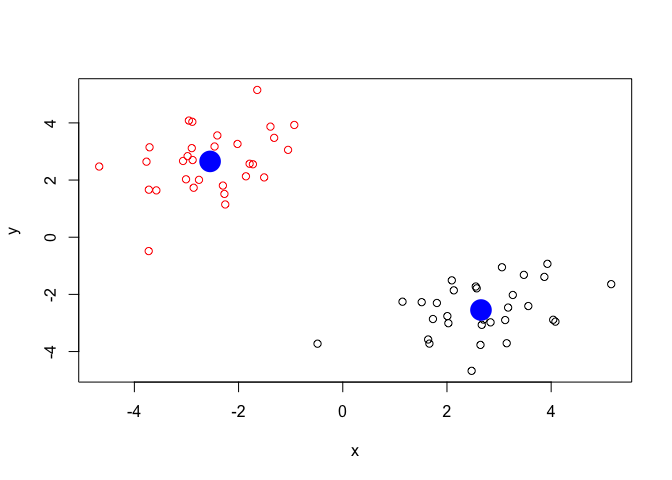
\includegraphics{Class-8_files/figure-latex/unnamed-chunk-6-1.pdf}

\hypertarget{hierarchical-clustering-in-r}{%
\subsection{Hierarchical clustering in
R}\label{hierarchical-clustering-in-r}}

The \texttt{hclust()} function is the main hierarchical clustering
method in R and it MUST BE PASSED THROUGH A MATRIX AS INPUT, not your
raw data!!!!

\begin{Shaded}
\begin{Highlighting}[]
\NormalTok{hc <-}\StringTok{ }\KeywordTok{hclust}\NormalTok{( }\KeywordTok{dist}\NormalTok{(x))  }\CommentTok{# this hopefully reveals patterns in your data}
\KeywordTok{plot}\NormalTok{(hc)}
\end{Highlighting}
\end{Shaded}

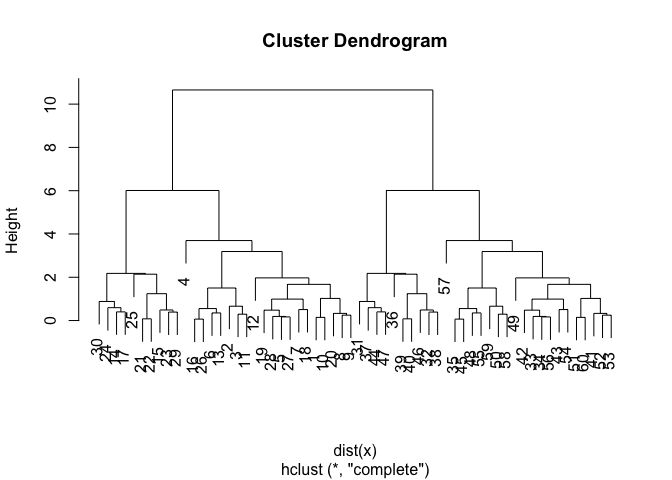
\includegraphics{Class-8_files/figure-latex/unnamed-chunk-7-1.pdf}

\begin{Shaded}
\begin{Highlighting}[]
\KeywordTok{plot}\NormalTok{(hc)}
\KeywordTok{abline}\NormalTok{(}\DataTypeTok{h=}\DecValTok{6}\NormalTok{, }\DataTypeTok{col=}\StringTok{"red"}\NormalTok{, }\DataTypeTok{lty=} \DecValTok{2}\NormalTok{)}\CommentTok{# makes a line above where you want to cut off the data}
\KeywordTok{abline}\NormalTok{(}\DataTypeTok{h=}\FloatTok{3.5}\NormalTok{, }\DataTypeTok{col=}\StringTok{"blue"}\NormalTok{, }\DataTypeTok{lty=} \DecValTok{2}\NormalTok{)}
\end{Highlighting}
\end{Shaded}

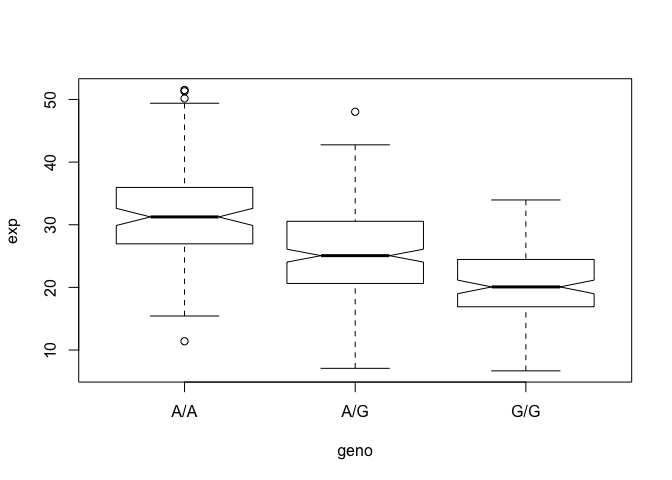
\includegraphics{Class-8_files/figure-latex/unnamed-chunk-8-1.pdf}

\begin{Shaded}
\begin{Highlighting}[]
\KeywordTok{cutree}\NormalTok{(hc, }\DataTypeTok{h=}\DecValTok{6}\NormalTok{)  }\CommentTok{# lists all the points below that line you cut}
\end{Highlighting}
\end{Shaded}

\begin{verbatim}
##  [1] 1 1 1 1 1 1 1 1 1 1 1 1 1 1 1 1 1 1 1 1 1 1 1 1 1 1 1 1 1 1 2 2 2 2 2 2 2 2
## [39] 2 2 2 2 2 2 2 2 2 2 2 2 2 2 2 2 2 2 2 2 2 2
\end{verbatim}

You can call cutree with \texttt{k} for the number of groups you want,
or with \texttt{h} for height

\begin{Shaded}
\begin{Highlighting}[]
\KeywordTok{cutree}\NormalTok{(hc, }\DataTypeTok{k=}\DecValTok{6}\NormalTok{) }\CommentTok{# having a lower cut off you see now you have 6 clusters}
\end{Highlighting}
\end{Shaded}

\begin{verbatim}
##  [1] 1 2 2 1 1 2 3 1 1 1 1 1 3 1 2 1 2 3 3 1 2 3 3 2 1 3 1 2 1 1 4 4 5 4 6 4 5 6
## [39] 6 5 4 6 6 5 4 5 4 6 4 4 4 4 4 6 5 4 4 5 5 4
\end{verbatim}

\hypertarget{linkage}{%
\subsection{Linkage}\label{linkage}}

\begin{Shaded}
\begin{Highlighting}[]
\CommentTok{# Step 1. Generate some example data for clustering}
\NormalTok{x <-}\StringTok{ }\KeywordTok{rbind}\NormalTok{(}
 \KeywordTok{matrix}\NormalTok{(}\KeywordTok{rnorm}\NormalTok{(}\DecValTok{100}\NormalTok{, }\DataTypeTok{mean=}\DecValTok{0}\NormalTok{, }\DataTypeTok{sd=}\FloatTok{0.3}\NormalTok{), }\DataTypeTok{ncol =} \DecValTok{2}\NormalTok{), }\CommentTok{# c1}
 \KeywordTok{matrix}\NormalTok{(}\KeywordTok{rnorm}\NormalTok{(}\DecValTok{100}\NormalTok{, }\DataTypeTok{mean=}\DecValTok{1}\NormalTok{, }\DataTypeTok{sd=}\FloatTok{0.3}\NormalTok{), }\DataTypeTok{ncol =} \DecValTok{2}\NormalTok{), }\CommentTok{# c2}
 \KeywordTok{matrix}\NormalTok{(}\KeywordTok{c}\NormalTok{(}\KeywordTok{rnorm}\NormalTok{(}\DecValTok{50}\NormalTok{, }\DataTypeTok{mean=}\DecValTok{1}\NormalTok{, }\DataTypeTok{sd=}\FloatTok{0.3}\NormalTok{), }\CommentTok{# c3}
 \KeywordTok{rnorm}\NormalTok{(}\DecValTok{50}\NormalTok{, }\DataTypeTok{mean=}\DecValTok{0}\NormalTok{, }\DataTypeTok{sd=}\FloatTok{0.3}\NormalTok{)), }\DataTypeTok{ncol =} \DecValTok{2}\NormalTok{))}
\KeywordTok{colnames}\NormalTok{(x) <-}\StringTok{ }\KeywordTok{c}\NormalTok{(}\StringTok{"x"}\NormalTok{, }\StringTok{"y"}\NormalTok{)}
\CommentTok{# Step 2. Plot the data without clustering}
\KeywordTok{plot}\NormalTok{(x)}
\end{Highlighting}
\end{Shaded}

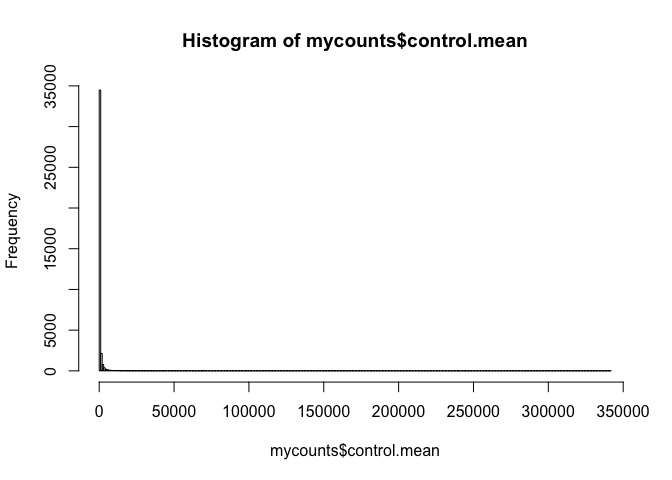
\includegraphics{Class-8_files/figure-latex/unnamed-chunk-11-1.pdf}

\begin{Shaded}
\begin{Highlighting}[]
\CommentTok{# Step 3. Generate colors for known clusters}
\CommentTok{# (just so we can compare to hclust results)}
\NormalTok{col <-}\StringTok{ }\KeywordTok{as.factor}\NormalTok{( }\KeywordTok{rep}\NormalTok{(}\KeywordTok{c}\NormalTok{(}\StringTok{"c1"}\NormalTok{,}\StringTok{"c2"}\NormalTok{,}\StringTok{"c3"}\NormalTok{), }\DataTypeTok{each=}\DecValTok{50}\NormalTok{) )}
\KeywordTok{plot}\NormalTok{(x, }\DataTypeTok{col=}\NormalTok{col)}
\end{Highlighting}
\end{Shaded}

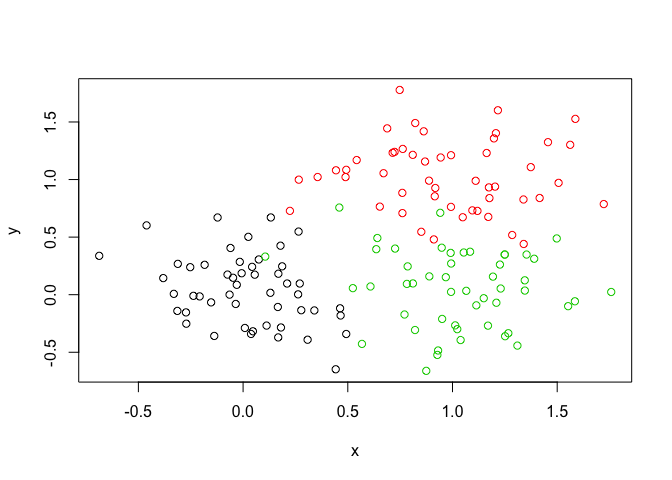
\includegraphics{Class-8_files/figure-latex/unnamed-chunk-11-2.pdf}

Q. Use the dist() for distance matrix, hclust(), plot() and cutree()
functions to return 2 and 3 clusters Q. How does this compare to your
known `col' groups?

\begin{Shaded}
\begin{Highlighting}[]
\NormalTok{hc <-}\StringTok{ }\KeywordTok{hclust}\NormalTok{(}\KeywordTok{dist}\NormalTok{(x))}
\KeywordTok{plot}\NormalTok{(hc)}
\end{Highlighting}
\end{Shaded}

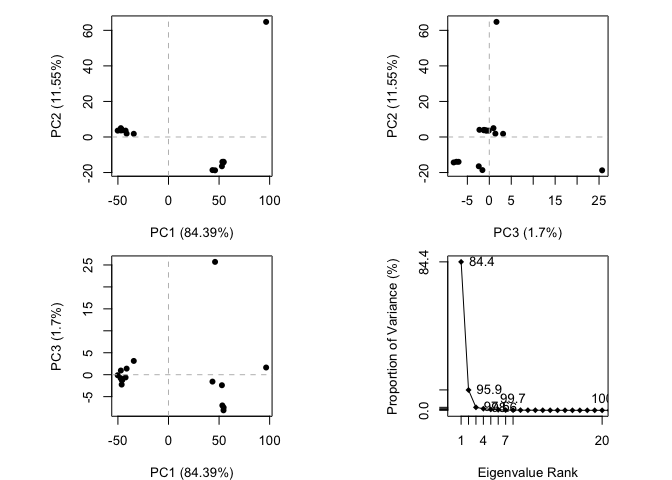
\includegraphics{Class-8_files/figure-latex/unnamed-chunk-12-1.pdf}

\begin{Shaded}
\begin{Highlighting}[]
\NormalTok{grps2 <-}\StringTok{ }\KeywordTok{cutree}\NormalTok{(hc, }\DataTypeTok{k=}\DecValTok{2}\NormalTok{)}
\NormalTok{grps3 <-}\StringTok{ }\KeywordTok{cutree}\NormalTok{(hc, }\DataTypeTok{k=}\DecValTok{3}\NormalTok{) }\CommentTok{#these are membership vectors}
\end{Highlighting}
\end{Shaded}

\begin{Shaded}
\begin{Highlighting}[]
\KeywordTok{table}\NormalTok{(grps2)}
\end{Highlighting}
\end{Shaded}

\begin{verbatim}
## grps2
##  1  2 
## 99 51
\end{verbatim}

\begin{Shaded}
\begin{Highlighting}[]
\KeywordTok{table}\NormalTok{(grps3)}
\end{Highlighting}
\end{Shaded}

\begin{verbatim}
## grps3
##  1  2  3 
## 45 54 51
\end{verbatim}

\begin{Shaded}
\begin{Highlighting}[]
\KeywordTok{plot}\NormalTok{(x, }\DataTypeTok{col=}\NormalTok{grps3) }\CommentTok{# color by the group distribution}
\end{Highlighting}
\end{Shaded}

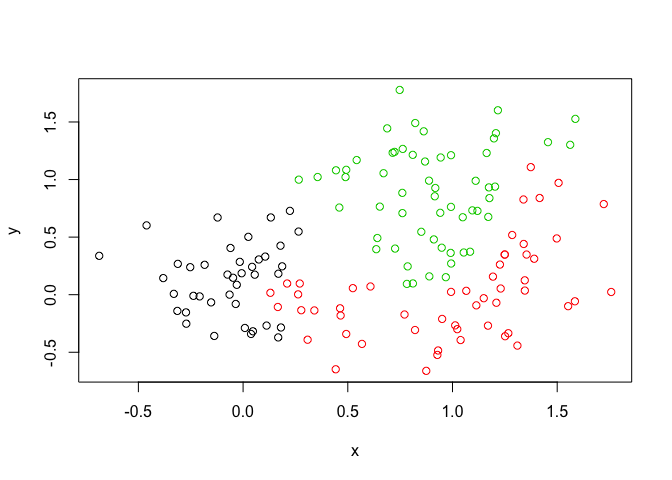
\includegraphics{Class-8_files/figure-latex/unnamed-chunk-15-1.pdf}

\begin{Shaded}
\begin{Highlighting}[]
\KeywordTok{table}\NormalTok{(grps3, col) }\CommentTok{#this is a cross table, using col from line 102, saying for group 1 all 42 points come from cluster 1, for group 2 most points come from cluster 3, for group 3 most points come from cluster 2 - so only group 1 is mostly right}
\end{Highlighting}
\end{Shaded}

\begin{verbatim}
##      col
## grps3 c1 c2 c3
##     1 45  0  0
##     2  5  4 45
##     3  0 46  5
\end{verbatim}

\hypertarget{principle-component-analysis-pca}{%
\section{Principle Component Analysis
(PCA)}\label{principle-component-analysis-pca}}

The main function in R for PCA is called \texttt{prcomp()}. Here we will
use PCA to examine the funny food that folks eat in the UK and N.
Ireland.

Import the CSV file first:

\begin{Shaded}
\begin{Highlighting}[]
\NormalTok{x <-}\StringTok{ }\KeywordTok{read.csv}\NormalTok{(}\StringTok{"UK_foods.csv"}\NormalTok{, }\DataTypeTok{row.names =} \DecValTok{1}\NormalTok{)}
\NormalTok{x}
\end{Highlighting}
\end{Shaded}

\begin{verbatim}
##                     England Wales Scotland N.Ireland
## Cheese                  105   103      103        66
## Carcass_meat            245   227      242       267
## Other_meat              685   803      750       586
## Fish                    147   160      122        93
## Fats_and_oils           193   235      184       209
## Sugars                  156   175      147       139
## Fresh_potatoes          720   874      566      1033
## Fresh_Veg               253   265      171       143
## Other_Veg               488   570      418       355
## Processed_potatoes      198   203      220       187
## Processed_Veg           360   365      337       334
## Fresh_fruit            1102  1137      957       674
## Cereals                1472  1582     1462      1494
## Beverages                57    73       53        47
## Soft_drinks            1374  1256     1572      1506
## Alcoholic_drinks        375   475      458       135
## Confectionery            54    64       62        41
\end{verbatim}

\begin{Shaded}
\begin{Highlighting}[]
\CommentTok{# Notice that X is the lable for the first column, but you want that to be the row names. You can fix that in the import function, with row.names=1}
\end{Highlighting}
\end{Shaded}

\begin{Shaded}
\begin{Highlighting}[]
\KeywordTok{barplot}\NormalTok{(}\KeywordTok{as.matrix}\NormalTok{(x), }\DataTypeTok{beside=}\NormalTok{T, }\DataTypeTok{col=}\KeywordTok{rainbow}\NormalTok{(}\KeywordTok{nrow}\NormalTok{(x)))}
\end{Highlighting}
\end{Shaded}

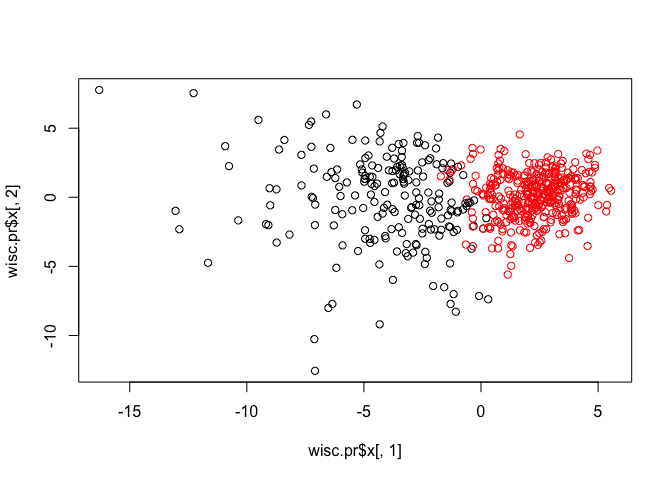
\includegraphics{Class-8_files/figure-latex/unnamed-chunk-18-1.pdf}

\begin{Shaded}
\begin{Highlighting}[]
\KeywordTok{pairs}\NormalTok{(x, }\DataTypeTok{col=}\KeywordTok{rainbow}\NormalTok{(}\DecValTok{10}\NormalTok{), }\DataTypeTok{pch=}\DecValTok{16}\NormalTok{)  }\CommentTok{#Makes a matrix of scatterplots}
\end{Highlighting}
\end{Shaded}

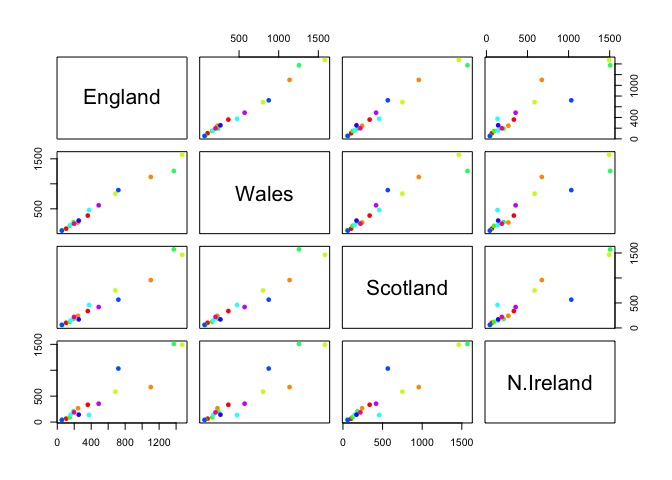
\includegraphics{Class-8_files/figure-latex/unnamed-chunk-19-1.pdf}

\#PCA to the rescue!

\begin{Shaded}
\begin{Highlighting}[]
\NormalTok{pca <-}\KeywordTok{prcomp}\NormalTok{(}\KeywordTok{t}\NormalTok{(x)) }\CommentTok{#taking the transpose of x makes the rows the column names}
\end{Highlighting}
\end{Shaded}

\begin{Shaded}
\begin{Highlighting}[]
\KeywordTok{summary}\NormalTok{(pca)}
\end{Highlighting}
\end{Shaded}

\begin{verbatim}
## Importance of components:
##                             PC1      PC2      PC3       PC4
## Standard deviation     324.1502 212.7478 73.87622 4.189e-14
## Proportion of Variance   0.6744   0.2905  0.03503 0.000e+00
## Cumulative Proportion    0.6744   0.9650  1.00000 1.000e+00
\end{verbatim}

\begin{Shaded}
\begin{Highlighting}[]
\KeywordTok{attributes}\NormalTok{(pca)}
\end{Highlighting}
\end{Shaded}

\begin{verbatim}
## $names
## [1] "sdev"     "rotation" "center"   "scale"    "x"       
## 
## $class
## [1] "prcomp"
\end{verbatim}

\begin{Shaded}
\begin{Highlighting}[]
\KeywordTok{plot}\NormalTok{( pca}\OperatorTok{$}\NormalTok{x[,}\DecValTok{1}\NormalTok{], pca}\OperatorTok{$}\NormalTok{x[,}\DecValTok{2}\NormalTok{] )}
\KeywordTok{text}\NormalTok{(pca}\OperatorTok{$}\NormalTok{x[,}\DecValTok{1}\NormalTok{], pca}\OperatorTok{$}\NormalTok{x[,}\DecValTok{2}\NormalTok{], }\KeywordTok{colnames}\NormalTok{(x), }\DataTypeTok{col=}\KeywordTok{c}\NormalTok{(}\StringTok{"black"}\NormalTok{, }\StringTok{"red"}\NormalTok{, }\StringTok{"blue"}\NormalTok{, }\StringTok{"darkgreen"}\NormalTok{))}
\end{Highlighting}
\end{Shaded}

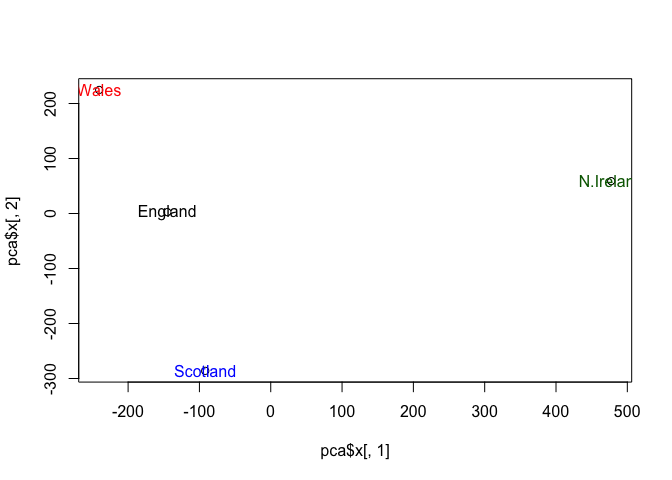
\includegraphics{Class-8_files/figure-latex/unnamed-chunk-23-1.pdf}

\end{document}
